%%% Ne pas modifier jusqu'à la ligne 25
\documentclass[a4paper,12pt]{book}
\usepackage[utf8]{inputenc}
\usepackage[french]{babel}
%%\usepackage{CJK}
\usepackage{yhmath}
\usepackage[left=2cm,right=2cm,top=3cm,bottom=2cm, headheight=1.5cm,headsep=1.5cm]{geometry}
%%\usepackage{CJKutf8}
\usepackage{amsfonts}
\usepackage{mathrsfs}
\usepackage{amsmath,amsfonts,amssymb,dsfont}
\usepackage{graphicx}
\usepackage{subfigure}
\usepackage{enumitem}		%\enumerate-resume
\usepackage[colorlinks=true,unicode={true},hyperindex=false, linkcolor=blue, urlcolor=blue]{hyperref}
\newcommand{\myref}[1]{\ref{#1} page \pageref{#1}}

\addto\captionsfrench{\def\tablename{Tableau}}  %légendes des tableaux
\renewcommand\thesection{\Roman{section}~-~} 
\renewcommand\thesubsection{\Roman{section}.\Alph{subsection}~-~} 
\renewcommand\thesubsubsection{\Roman{section}.\Alph{subsection}.\arabic{subsubsection}~-~} 

\newcommand{\conclusion}[1]{\newline \centerline{\fbox{#1}}}

\setcounter{secnumdepth}{3}
\parindent=0pt

\usepackage{fancyhdr}
\pagestyle{fancy}

\lhead{SJTU-ParisTech} 
%%%%%%%%%%%%%%%%%%%%%%%%%%%%%%%%%%
\chead{TR9}
\rhead{Daniel 518261910024}

\begin{document}
\renewcommand{\labelitemi}{$\blacktriangleright$}
\renewcommand{\labelitemii}{$\bullet$}


\section{synthèse du chapitre 4}
\subsection{Deux types de configurations}
% \begin{table}[h]
%     \begin{center}
%         \begin{tabular}{l|l}
%         \hline
%          définition   &  cool   \\ \hline  
%         \end{tabular}
%     \end{center}
% \end{table}
\begin{itemize}
    \item Configuration de la lame d'air
    
    Définition: Lorsque les deux miroirs plans $M_1$ et $M_2$ d'un interféromètre de Michelson sont orthogonaux mais ne 
    sont pas symétriques par rapport à $(S_p)$, l'interféromètre est équivalent à une lame d'air 
    d'épaisseur e comprise entre $M_2$ et $M_1^{'}$(l'image du $M_1$)

    \item Configuration de la coin d'air
    
    Définition: Lorsque les deux miroirs plans $M_1$ et $M_2$ d'un interféromètre de Michelson ne sont pas parfaitement
    orthogonaux , l'interféromètre est équivalent à un coin d'air d'angle $\alpha$(l'angle entre $M_1^{'}$ et $M_2$.
\end{itemize}
\begin{figure}[htbp]
    \centering
    \subfigure[Configuration de la lame d'air]{
    \begin{minipage}[t]{0.5\linewidth}
    \centering
    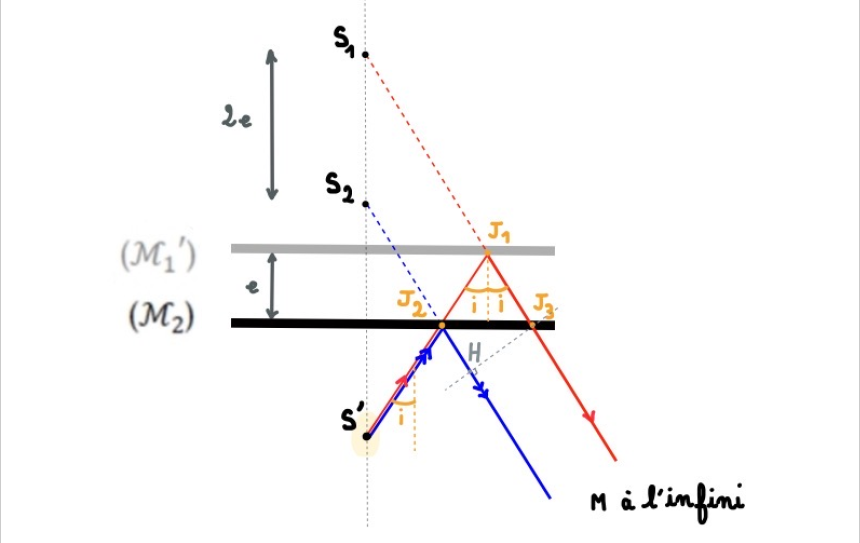
\includegraphics[scale=0.7]{lame.png}
    %\caption{fig1}
    \end{minipage}%
    }%
    \subfigure[Configuration de la coin d'air]{
    \begin{minipage}[t]{0.5\linewidth}
    \centering
    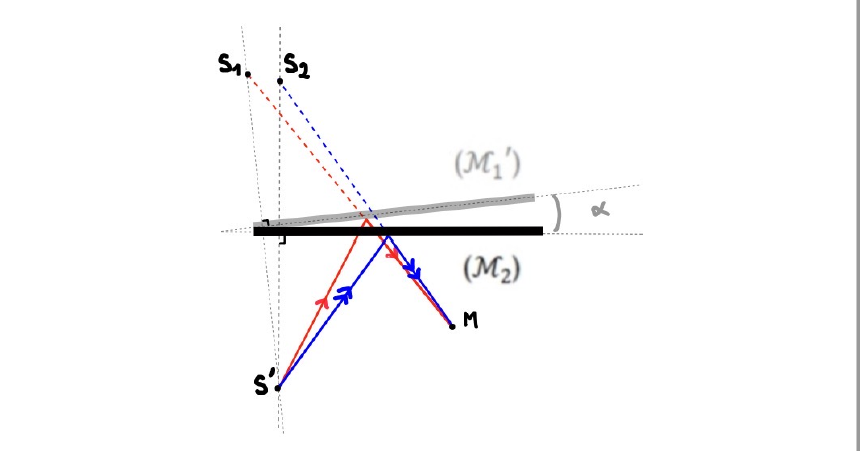
\includegraphics[scale=0.7]{coin.png}
    %\caption{fig2}
    \end{minipage}%
    }%
    \centering
    %\caption{ pics}
    \caption{Deux types de configurations}
\end{figure}


\subsection{une source ponctuelle}
\subsubsection{lame d'air}
\begin{itemize}
    \item distance finie
        \begin{itemize}
            \item Champ d'interférences: hyperboloïdes avec les foyers: les sources secondaires
                    $S_1$ et $S_2$, l'axe de révolution $(S_1S_2)$
            \item Délocalisation: En plaçant l'ecran d'observation par parallèle aux miroirs, les franges sont les cercles. 
                    Si l'on déplace l'écran parallèlement, la figure d'interférences varie 
        \end{itemize}
\end{itemize}
\subsubsection{coin d'air}
\begin{itemize}
    \item distance finie
        \begin{itemize}
            \item Champ d'interférences: hyperboloïdes avec les foyers: les sources secondaires
                    $S_1$ et $S_2$, l'axe de révolution $(S_1S_2)$
            \item Délocalisation: En plaçant l'ecran d'observation par parallèle à $M_2$($(S_1S_2)$ est pratiquement parallèle à $M_2$), les franges sont les hyperboles 
            si l'on fait l'observation proche des miroirs, et quasi-rectilignes à une grande distance. 
                    Si l'on déplace l'écran parallèlement, la figure d'interférences varie 
        \end{itemize}
\end{itemize}
\subsection{une source étendue}
\subsubsection{lame d'air}
\begin{itemize}
    \item Localisation: Localisées à l'infini. Lorsque on fait l'observation à distance finie, les franges sont brouillées si l'on décompose la source étendue mentalement 
    en des sources ponctuelles.
    \item Franges d'égale inclinaison. La différence de marche à l'infini ne dépend 
          que de l'angle d'incidence i des rayons
    \item Différence de march: $\delta(M_{\infty})=2e\cos{i}$
    \item Comparaison avec une source ponctuelle: la même figure d'interférences, mais plus contrastée
    \item Figure d'interférences: Anneaux de Haidinger avec le centre $F^{'}$
    \item Application: Mesurer des distances infiniment petites avec une bonne précision
\end{itemize}

\subsubsection{coin d'air}
\begin{itemize}
    \item Localisation: Localisées au voisinage des miroirs, avec incidence quasi-normale. La figure d'interférences perd en contraste 
          au fur et à mesure que la source est élargie et l'écran est éloigné des miroirs.
    \item Franges d'égale épaisseur. La différence de march dépend que l'épaisseur locale du point étudié au voisinage du miroir et avec incidence 
          normale. Chaque couple des sources secondaires imaginaires donne la même figure d'interférences.
    \item Différence de march(incidence quasi-normale): $\delta(M)=2\alpha x_M$
    \item Comparaison avec une source ponctuelle: la même figure d'interférences, aussi contrastée, et plus lumineuse
    \item Figure d'interférences: des droites parallèles entre elles, perpendiculaire à l'axe $Ox$, parallèle à l'arête du coin d'air
    \item Application: Mesure de chemin optique
\end{itemize}
\begin{figure}[htbp]
    \centering
    \subfigure[La figure d'interferences de la lame d’air à l'infini]{
    \begin{minipage}[t]{0.5\linewidth}
    \centering
    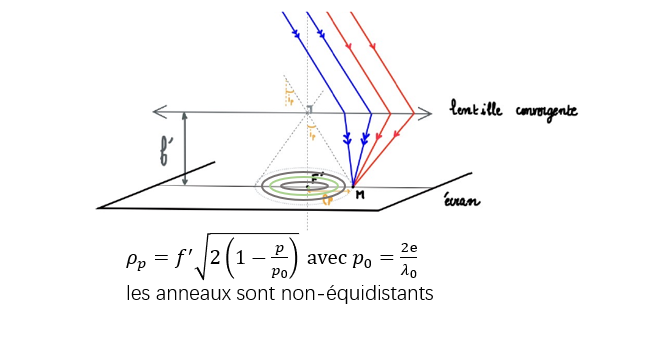
\includegraphics[scale=0.8]{lameinfini.png}
    %\caption{fig1}
    \end{minipage}%
    }%
    \subfigure[La figure d'interferences de la coin d'air au voisinage des miroirs]{
    \begin{minipage}[t]{0.5\linewidth}
    \centering
    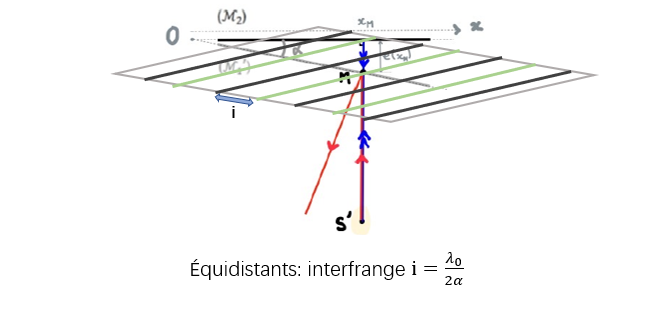
\includegraphics[scale=0.8]{coinvoisinage.png}
    %\caption{fig2}
    \end{minipage}%
    }%
    \centering
    %\caption{ pics}
    \caption{Figure d'interferences}
\end{figure}


\end{document}